\documentclass[11pt, letterpaper]{article}
\usepackage[utf8]{inputenc}
\usepackage[letterpaper, margin=1in]{geometry}
\usepackage{amsmath}
\usepackage{amssymb}
\usepackage{amsthm}
\usepackage{graphicx}
\usepackage[font=scriptsize]{caption}
\usepackage{subcaption}
\graphicspath{ {.} }
\captionsetup{justification=raggedright, singlelinecheck=false}


\title{Homework 2}
\author{Ryan Tang}
\date{October 13th 2022}

\begin{document}
\maketitle

\section{Exercise 11.3}
Some notations to set it straight and lots of indexing are presented. Assume $x \in \{0,1\}^D, j = 1 \dots D$ a binary vector. The full data matrix is then $\mathbf{X} \in \mathbb{R}^{N \times D}$, with the assumption that each individual $x_i, i = 1 \dots N$ are $iid$ observation for the sake of the likelihood function. I will also introduce an indicator $z_i \in \{0, 1\}^K$, where $\mathbf{Z} = \{z_i\}_{i=1\dots N}$. Lastly, we would like to assume a mixture of the Bernoulli model. Thus, with $K$ unknown mixture, each binary value within the $x$ vector follows a Bernoulli distribution, $x_{kj} \thicksim Bernoulli(p_{kj})$, and the mixture follows an unknown distribution $\pi(k)$. With the above notation, we can write the complete log data likelihood and the EM auxiliary function as follow.

\begin{align*}
    \ell(\theta) &= \sum_i \log p(x_i, z_i|\theta) \\
    p(x_i, z_i|\theta) &= \prod_k [\pi_k p(x_i|\theta_k)]^{z_{ik}} \\
    Q(\theta, \theta^{t-1}) &= \mathbb{E}[\ell(\theta)|\mathbf{X}, \theta^{t-1}] \\
        &= \sum_i \sum_k r_{ik} \ln \pi_k + \sum_i \sum_k r_{ik} \ln p(x_i|\theta_k) \\ 
\end{align*}

Now take the derivative of the auxiliary function for $p_{kj}$, and we arrive at the following result.

\begin{align*}
    \frac{\partial}{\partial p_{kj}}Q &= \sum_i r_{ik} [\frac{x_{ij}}{p_{kj}} - \frac{1-x_{ij}}{1-p_{kj}}] = 0 \\
        & \sum_i r_{ik} [x_{ij}(1-p_{kj}) - (1-x_{ij})p_{kj}] = 0 \\
        & \sum_i (x_{ij} - p_{kj}) = 0 \\
    p_{kj} &= \frac{\sum_i r_{ik} x_{ij}}{\sum_i r_{ik}}
\end{align*}

If we look at it from the Bayesian perspective, putting a prior on $p_{kj} \thicksim Beta(a, b)$, we can derive the MAP solutions from the MLE solutions.

\begin{align*}
    \ell(\theta)_{MAP} &\propto \sum_i \log p(x_i, z_i|\theta) + \log p(\theta) \\
    Q(\theta, \theta^{t-1}|D) &= \sum_i \sum_k r_{ik} \ln \pi_k + \sum_i \sum_k r_{ik} \ln p(x_i|\theta_k) + \log p(\theta) \\
    \frac{\partial}{\partial p_{kj}}Q &= 
            \sum_i r_{ik} [\frac{x_{ij}}{p_{kj}} - \frac{1-x_{ij}}{1-p_{kj}}] + \frac{a-1}{p_{kj}} - \frac{b-1}{1-p_{kj}} = 0 \\
        & \sum_i r_{ik} [x_{ij}(1-p_{kj}) - (1-x_{ij})p_{kj}] + (a-1)(1-p_{kj}) - (b-1)p_{kj} = 0 \\
        & \sum_i r_{ik} x_{ij} - \sum_i r_{ik} p_{kj} + (a-1) - (a+b+2) p_{kj} = 0 \\
        & p_{kj} = \frac{(\sum_i r_{ik} x_{ij}) + a - 1}{(\sum_i r_{ik}) + a + b - 2}
\end{align*}


\section{Exercise 11.5}
For fitting the GMM using gradient descent, we can directly derive the gradient through the log-likelihood.
\begin{align*}
    \ell(\theta) &= \sum_i \log p(x_i|\theta) \\
    p(x|\theta) &= \sum_k \pi_k \mathcal{N}(x|\mu_k, \Sigma_k) \\
    \frac{\partial}{\partial \mu_k} \ell(\theta) &= \sum_i \frac{\partial}{\partial \mu_k} \log p(x_i|\theta) \\
        &= \sum_i \frac{\partial}{\partial \mu_k} \log [\sum_k \pi_k \mathcal{N}(x_i|\mu_k, \Sigma_k)] \\
        &= \sum_i \frac{\frac{\partial}{\partial \mu_k} \sum_{k} \pi_{k} \mathcal{N}(x_i|\mu_{k}, \Sigma_{k})}{\sum_{k'} \pi_{k'} \mathcal{N}(x_i|\mu_{k'}, \Sigma_{k'})} \\
        &= \sum_i
            \frac{ \pi_{k} \mathcal{N}(x_i|\mu_{k}, \Sigma_{k})}
                 {\sum_{k'} \pi_{k'} \mathcal{N}(x_i|\mu_{k'}, \Sigma_{k'})}
            \frac{\partial}{\partial \mu_k} [-\frac{1}{2}(x_i-\mu_k)^{\intercal}\Sigma^{-1}(x_i-\mu_k)] \\
        &= \sum_i r_{ik} \Sigma_{k}^{-1} (x_i - \mu_k)
\end{align*}

And the gradient for the generic $\pi_k$ without any constraints is given below.
\begin{align*}
    \frac{\partial}{\partial \pi_k} \ell(\theta) &= 
        \sum_i \frac{\frac{\partial}{\partial \pi_k} \sum_{k} \pi_{k} \mathcal{N}(x_i|\mu_{k}, \Sigma_{k})}
                    {\sum_{k'} \pi_{k'} \mathcal{N}(x_i|\mu_{k'}, \Sigma_{k'})} \\
        &= \sum_i \frac{\mathcal{N}(x_i|\mu_{k}, \Sigma_{k})}{\sum_{k'} \pi_{k'} \mathcal{N}(x_i|\mu_{k'}, \Sigma_{k'})} \\
        &= \sum_i r_{ik} \frac{1}{\pi_k}
\end{align*}

Now, if we use softmax to handle the constraint $\sum_k \pi_k = 1$, we can rewrite the above derivative with respect $w_k$ as the following.
\begin{align*}
    \pi_k &= \frac{e^{w_k}}{\sum_{k'} e^{w_{k'}}} \\
    \frac{\partial}{\partial w_k} \ell(\theta) &= 
        \sum_i \frac{\frac{\partial}{\partial w_k} \sum_{k} \pi_{k} \mathcal{N}(x_i|\mu_{k}, \Sigma_{k})}
                    {\sum_{k'} \pi_{k'} \mathcal{N}(x_i|\mu_{k'}, \Sigma_{k'})} \\
        &= \sum_i [
            \frac{\pi_k \mathcal{N}(x_i|\mu_{k}, \Sigma_{k})}{\sum_{k'} \pi_{k'} \mathcal{N}(x_i|\mu_{k'}, \Sigma_{k'})} (1-\pi_k)
            - \sum_{j \neq k} \frac{\pi_j \mathcal{N}(x_i|\mu_{j}, \Sigma_{j})}{\sum_{k'} \pi_{k'} \mathcal{N}(x_i|\mu_{k'}, \Sigma_{k'})} \pi_k
        ] \\
        &= \sum_i [r_{ik}(1-\pi_k) - (\sum_{j\neq k} r_{ij}) \pi_k] \\
        &= \sum_i [r_{ik} - \pi_k(r_{ik} + \sum_{j \neq k} r_{ij})] \\
        &= \sum_i r_{ik} - \pi_k
\end{align*}

Following the same pattern of taking the derivative to $\Sigma_k$, we arrive at the following gradient after some messy linear algebra.
\begin{align*}
    \frac{\partial}{\partial \Sigma_{k}} \ell(\theta) &=
        -\frac{1}{2} \sum_i r_{ik} [\Sigma_k^{-1} - \Sigma_k^{-1}(x_i-\mu_k)(x_i-\mu_k)^{\intercal}\Sigma_k^{-1}] \\
\end{align*}

By imposing the symmetric positive definite constraints on the $\Sigma_k = RR^{\intercal}$ using Cholesky, we can arrive at the following gradient.
\begin{align*}
    \frac{\partial}{\partial R_{k}} \ell(\theta) &=
        \sum_i \frac{\frac{\partial}{\partial R_{k}} \sum_{k} \pi_{k} \mathcal{N}(x_i|\mu_{k}, \Sigma_{k})}
                    {\sum_{k'} \pi_{k'} \mathcal{N}(x_i|\mu_{k'}, \Sigma_{k'})} \\
        &= -\sum_i r_{ik} [R_k^{-T} - R_k^{-1}(x_i-\mu_k)(x_i-\mu_k)^{\intercal}]
\end{align*}


\section{Exercise 11.7}
Given the data, we like to optimize the following log-likelihood for this simple GMM.
\begin{align*}
    \theta^{(t)} &= \mathop{\arg\max}_{\theta} \mathbb{E}[\ell(\theta)|X, \theta^{(t-1)}] \\
        &= \mathop{\arg\max}_{\theta} \sum_i \sum_k r_{ik} \ln \pi_k + \sum_i \sum_k r_{ik} \ln \mathcal{N}(x_i|\mu_k, \Sigma_{k}) \\
    \pi_k &= \frac{\sum_i r_{ik}}{N} \\
    \mu_k &= \frac{\sum_i r_{ik}x_i}{\sum_i r_{ik}}
\end{align*}
Hence the new values are $\mu_1 = \frac{5}{1.4}$, $\mu_2 = \frac{26}{1.6}$, $\pi_1 = \frac{1.4}{3}$, and $\pi_2 = \frac{1.6}{3}$.


\section{Exercise 11.9}
The converged cluster means would look like the following graph using the iterative algorithm starting with those two circle positions.
\begin{figure*}[!h]
  \centering
  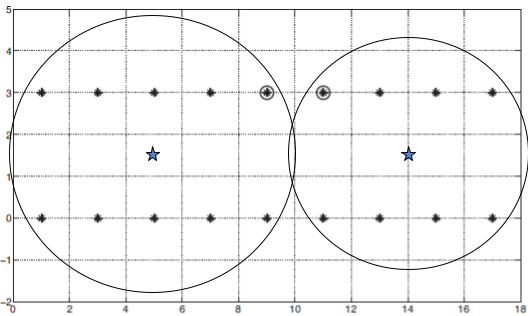
\includegraphics[width=0.7\textwidth]{11.9.png}
  \captionsetup{justification=centering}
  \caption{The Final K-Means Cluster}
\end{figure*}


\section{Exercise 11.14}
Sorry, got stuck on this one :(


\section{Exercise 11.15}
Some notations. $z_i$ is the true value never observed on the right tail. We observed the censored value $c_i$, which is strictly less than the true value. Assuming $z_i = \mu_i + \sigma \epsilon_i$ follows an addition error term, where $\epsilon_i \thicksim \mathcal{N}(0, 1)$, we can derive the following properties.
\begin{align*}
    \mathbb{E}[z_i|z_i \geq c_i] &= \mathbb{E}[\mu_i + \sigma \epsilon_i|\mu_i + \sigma \epsilon_i \geq c_i] \\
        &= \mu_i + \sigma \mathbb{E}[\epsilon_i | \epsilon_i \geq u_i] && u_i = \frac{c_i-\mu_i}{\sigma} \\
        &= \mu_i + \sigma \int \epsilon_i p(\epsilon_i|\epsilon \geq u_i) d\epsilon_i \\
        &= \mu_i + \sigma \frac{1}{1 - p(\epsilon_i \leq u_i)} \int \epsilon_i p(\epsilon_i, \epsilon_i \geq u_i) d\epsilon_i \\
        &= \mu_i + \sigma \frac{1}{1 - p(\epsilon_i \leq u_i)} \int_{u_i}^{\infty} \epsilon_i p(\epsilon_i) d\epsilon_i
            && \int_b^c w\mathcal{N}(w|0,1) dw = \mathcal{N}(b|0, 1) - \mathcal{N}(c|0, 1) \\
        &= \mu_i + \sigma \frac{1}{1 - p(\epsilon_i \leq u_i)} [\mathcal{N}(u_i|0, 1) - \mathcal{N}(\infty|0, 1)] \\
        &= \mu_i + \sigma \frac{\mathcal{N}(u_i|0, 1)}{1 - p(\epsilon_i \leq u_i)} \\
        &= \mu_i + \sigma H(u_i) && H = \frac{\phi(u)}{1 - \Phi(u)} \\
\end{align*}

For $\mathbb{E}[z_i^2|z_i\geq c_i]$, we need to expand the Gaussian integral trick again.
\begin{align*}
     \frac{d^2}{d^2w} \mathcal{N}(w|0,1) &= \frac{d}{dw} -w\mathcal{N}(w|0,1) \\
        &= -\mathcal{N}(w|0,1) + w^2\mathcal{N}(w|0,1) \\
    w^2\mathcal{N}(w|0,1) &= \mathcal{N}(w|0,1) -(\frac{d}{dw} w\mathcal{N}(w|0,1)) \\
    \int_a^{\infty} w^2\mathcal{N}(w|0,1) &= \int_a^{\infty} \mathcal{N}(w|0,1) -(\frac{d}{dw} \int_a^{\infty} w\mathcal{N}(w|0,1)) \\
        &= 1 - \Phi(a) - \frac{d}{dw} \mathcal{N}(a|0,1) \\
        &= 1 - \Phi(a) + a \mathcal{N}(a|0,1) \\ \\
    \mathbb{E}[z_i^2|z_i \geq c_i] &= \mathbb{E}[\mu_i^2 + \sigma^2\epsilon_i^2 + 2\mu_i\sigma\epsilon_i|\epsilon_i \geq u_i] \\
        &= \mu_i^2 + \sigma^2\mathbb{E}[\epsilon_i^2|\epsilon_i \geq u_i] + 2\mu_i\sigma\mathbb{E}[\epsilon_i|\epsilon_i \geq u_i] \\
        &= \mu_i^2 + \sigma^2(1+\frac{c_i-\mu_i}{\sigma}H(u_i)) + 2\mu_i\sigma H(u_i) \\
        &= \mu_i^2 + 2\mu_i\sigma H(u_i) + \sigma^2 + \sigma(c_i-\mu_i)H(u_i) \\
        &= \mu_i^2 + \sigma^2 + H(u_i)\sigma(c_i + \mu_i)
\end{align*}


\end{document}